\documentclass{uebblatt}

\begin{document}

\maketitle{7}

\begin{aufgabe}{Dichtheit ganzzahliger Linearkombinationen}
Sei~$x$ eine irrationale reelle Zahl. Zeige: $\operatorname{span}_\ZZ(1,x)$
liegt dicht in~$\RR$.
\end{aufgabe}

\begin{aufgabe}{Auf den Spuren Fermats}
Sei~$K$ ein Zahlkörper.
\begin{enumerate}
\item Sei~$m \geq 0$ eine zur Klassenzahl~$h_K$
teilerfremde Zahl. Sei~$\aaa \subseteq \O_K$ ein Ideal. Zeige: Ist~$\aaa^m$ ein
Hauptideal, so ist auch~$\aaa$ ein Hauptideal.
\item Gelte in~$\O_K$ die Identität~$z^p = x_1 \cdots x_n$,
wobei die~$x_i$ paarweise teilerfremd sind. Zeige: Ist~$h_K = 1$,
so sind die~$x_i$ bis auf Einheiten~$p$-te Potenzen.

{\tiny\emph{Hinweis.} Die Behauptung gilt in allgemeinen faktoriellen
Ringen.\par}
\item Zeige dieselbe Behauptung wie in~c) unter der schwächeren Voraussetzung~$p \nmid h_K$.
\item Zeige: Um Fermats großen Satz zu beweisen, genügt es, ihn für primzahlige
Exponenten und für den Exponent~4 zu beweisen.
\end{enumerate}
\end{aufgabe}

\begin{aufgabe}{Verzweigung von Primidealen}
Sei~$K = \QQ[\sqrt[3]{2}]$. Es ist~$(1,\sqrt[3]{2},\sqrt[3]{2}^2)$ eine
Ganzheitsbasis von~$\O_K$. Bestimme das Verzweigungsverhalten der
Primzahlen~$2, 3, 5$ und~$11$ in~$\O_K$.
\end{aufgabe}

\begin{aufgabe}{Mumfords Schatzkarte}
Die unten stehende Skizze visualisiert die Primideale von~$\ZZ[X]$.
Was möchte sie dir mitteilen? Untersuche folgende Fragen:
\begin{enumerate}
\item Welche Primideale sind jeweils zu vertikalen Linien gruppiert? Wieso?
\item Was hat die mit~"`$[(X^2+1)]$"' beschriftete Kurve mit dem
Verzweigungsverhalten von Primzahlen in~$\ZZ[i]$ zu tun?
\item Kannst du auf analoge Art und Weise die Primideale von~$\O_K$ aus
Aufgabe~2 visualisieren? Deine Skizze sollte aus zwei übereinander liegenden
Kurven bestehen, wobei die untere Kurve einfach die gerade Linie der Primideale
von~$\ZZ$ sein sollte.
\end{enumerate}
\centering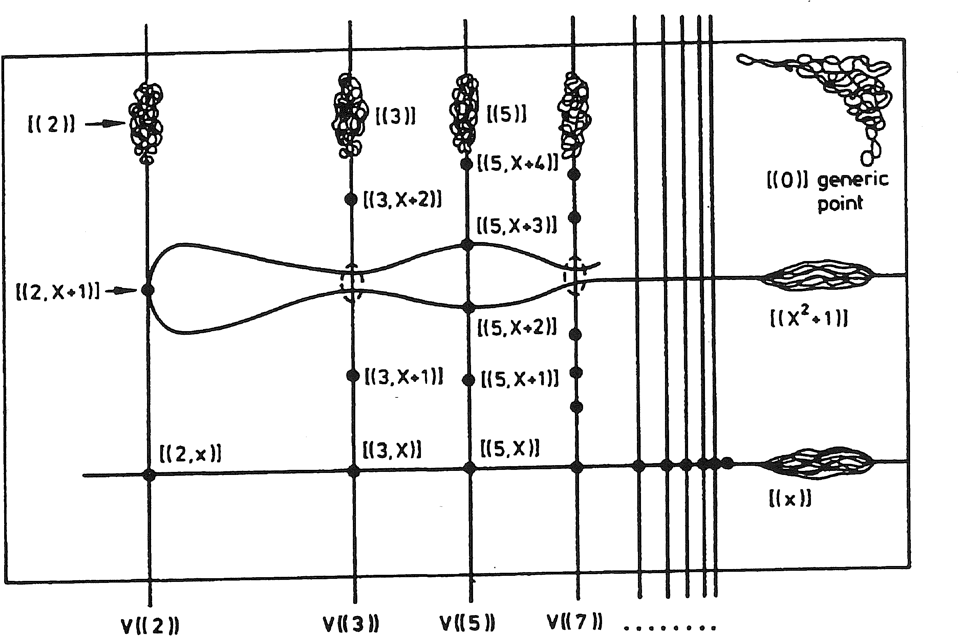
\includegraphics[width=0.6\textwidth]{images/mumfords-treasure-map}\par
\end{aufgabe}

\end{document}
